% =====================================================================
%  Fundamentals of Deep Learning — Class 7 (5 August)
%  Topic (course plan): Deep Networks
%  Subtopics: SNN to FNN, Universal Function Approximation
%
%  Sources: Prince, Understanding Deep Learning (2023), Ch. 4;
%           Bishop & Bishop, Deep Learning (2024), Ch. 6.
%  Figures: official vector PDFs from the authors' repositories,
%  used with attribution; teaching sequence follows Prince Ch. 4.
%
%  Compile:  xelatex main.tex   (run twice)
% =====================================================================
\documentclass[aspectratio=169, 11pt]{beamer}

\usetheme{metropoliscustom}

\usepackage{graphicx}
\graphicspath{{Class07_Deep_Networks_Universal_Approximation/figs_official/}{figs_official/}}
\usepackage{amsmath, amssymb}
\usepackage{bm}
\usepackage{tikz}
\usetikzlibrary{arrows.meta, positioning, calc}
\tcbuselibrary{skins}

\definecolor{shc}{HTML}{341651}    % shallow side (indigo)
\definecolor{dpc}{HTML}{800000}    % deep side (maroon)

% ---- parallel strip: Shallow (left) vs Deep (right)
\newcommand{\shpar}[2]{%
  \vfill
  {\footnotesize
  \begin{tcolorbox}[enhanced, sidebyside, sidebyside align=top,
                    lefthand ratio=0.485,
                    segmentation style={shc!35, line width=0.6pt},
                    colback=shc!5, colframe=shc!35, boxrule=0.5pt,
                    arc=1.5mm, left=2mm, right=2mm, top=0.8mm, bottom=0.8mm]
    {\color{shc}\textbf{SHALLOW}}\;\; #1
  \tcblower
    {\color{dpc}\textbf{DEEP}}\;\; #2
  \end{tcolorbox}}%
  \vspace{0.6em}%
}

\newcommand{\figsource}[1]{{\scriptsize\color{mcMuted} #1}}

% =====================================================================
\title{Deep Networks}
\subtitle{From Shallow to Feedforward, and Universal Approximation}
\author{Fundamentals of Deep Learning \ \textperiodcentered\ Class 7}
\institute{Prof.~Nirav Bhatt}
\date{5 August}

\footleft{Fundamentals of Deep Learning}
\footright{Deep Networks}
\titlelogos{}

\begin{document}

\maketitle

\begin{frame}{Outline}
  \tableofcontents
\end{frame}

% =====================================================================
\section{Composing Networks}
% =====================================================================

\begin{frame}{Where the shallow network left us}
  \begin{itemize}
    \item A shallow network is a linear read-out over
          \alert{learned features} $h_d=\mathrm{a}[\theta_{d0}
          +\theta_{d1}x]$ (Classes~5--6)
    \item With enough hidden units it is a
          \alert{universal approximator} --- but the number of
          units may be enormous
    \item Question for today: what if we feed the output of
          one network into the \alert{input of another}?
  \end{itemize}
  \vspace{0.3em}
  \begin{redhighlight}
    Stacking shallow networks gives a \alert{deep network}.
    The same building block, composed --- and far more
    efficient.
  \end{redhighlight}
\end{frame}

\begin{frame}{An intuition: solve a big problem in stages}
  \begin{itemize}
    \item A shallow network must map raw inputs to the answer
          in \alert{one leap} --- every hidden unit works
          directly on $x$
    \item A deep network solves the problem in
          \alert{stages}: layer~1 extracts simple features,
          layer~2 combines them into richer ones, and so on
    \item Reading is the analogy: \alert{strokes $\to$
          letters $\to$ words $\to$ meaning}. Nobody jumps
          from ink to meaning in a single step
    \item Each stage is \emph{easy} because it builds on the
          stage before --- the difficulty is \alert{spread
          across depth}
  \end{itemize}
  \shpar{one leap: raw input $\to$ answer}
        {staged: input $\to$ features $\to$ features of
         features $\to$ answer}
\end{frame}

\begin{frame}{Composing two networks}
  \centering
  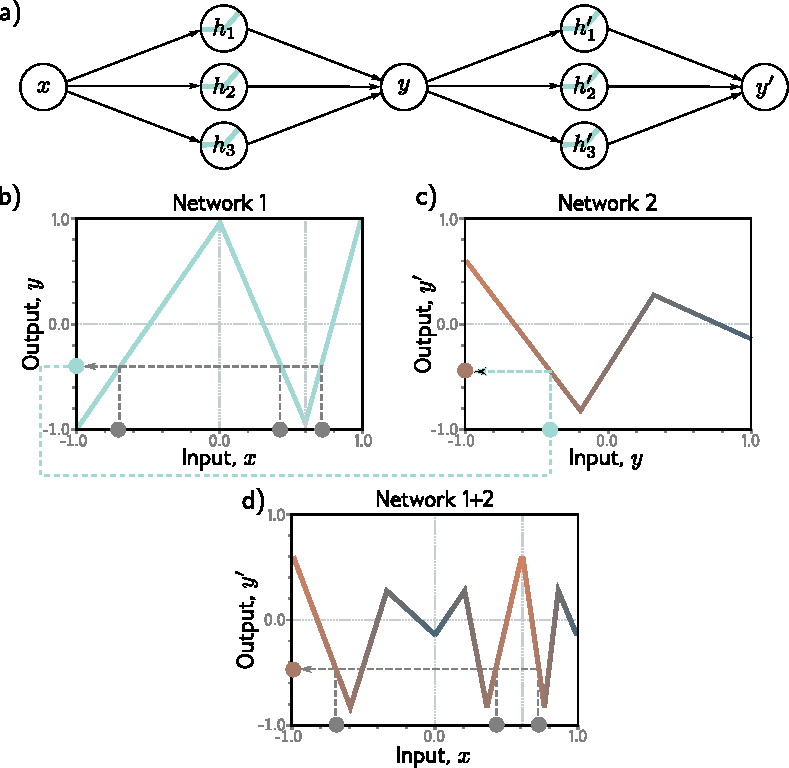
\includegraphics[height=0.60\textheight]{DeepConcat}
  \\[0.1em]
  \figsource{Prince (2023), Fig.~4.1: network~1 (left) feeds
  network~2 (right). Each is piecewise linear; their
  composition is piecewise linear with \emph{more} joints.}
\end{frame}

\begin{frame}{The folding analogy}
  \begin{columns}[T, onlytextwidth]
    \begin{column}{0.52\textwidth}
      \centering
      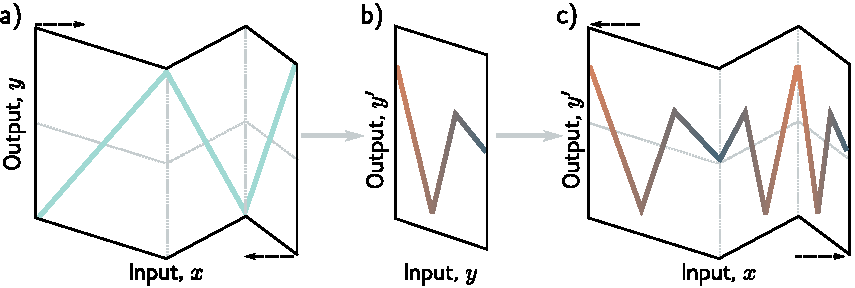
\includegraphics[width=\linewidth]{DeepFold}
      \\[0.1em]
      \figsource{Prince (2023), Fig.~4.3.}
    \end{column}
    \hfill
    \begin{column}{0.44\textwidth}
      \vspace{0.2em}
      \begin{itemize}\setlength{\itemsep}{1pt}
        \item The first network \alert{folds} input space
              back onto itself
        \item The second acts on the folded space --- one of
              its regions maps to \alert{several} input
              regions
        \item Folding is why depth multiplies regions instead
              of merely adding them
      \end{itemize}
    \end{column}
  \end{columns}
  \shpar{joints add: $D$ units $\to$ $D{+}1$ regions}
        {folding \emph{multiplies} regions across layers}
\end{frame}

\begin{frame}{Composing in two dimensions}
  \centering
  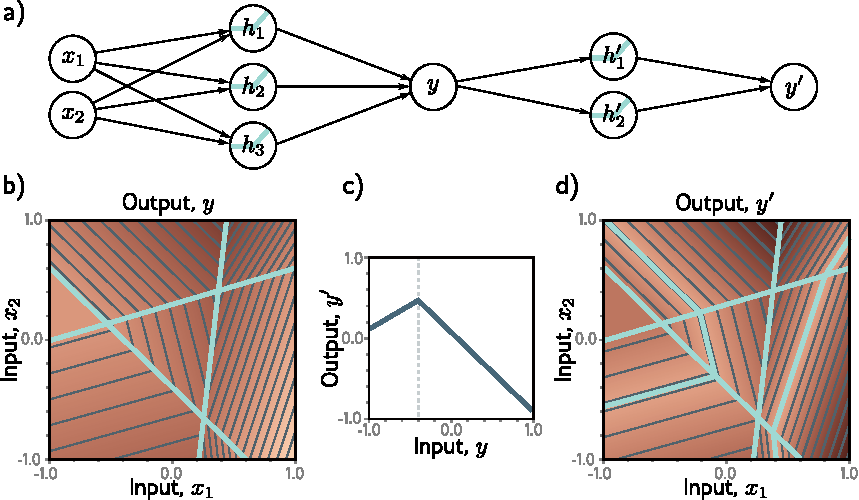
\includegraphics[height=0.62\textheight]{DeepTwoLayer2D}
  \\[0.1em]
  \figsource{Prince (2023), Fig.~4.2: composing networks with
  a 2D input; the second network re-uses the first network's
  convex regions to build a more intricate partition.}
\end{frame}

% =====================================================================
\section{The Deep Network}
% =====================================================================

\begin{frame}{Two hidden layers, one equation}
  \begin{columns}[T, onlytextwidth]
    \begin{column}{0.5\textwidth}
      \centering
      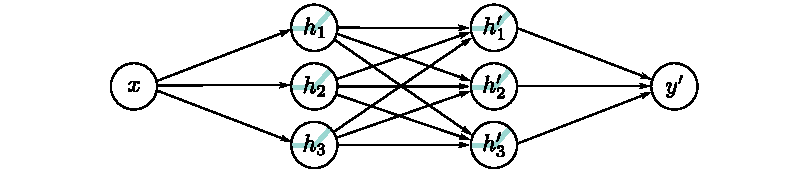
\includegraphics[width=0.95\linewidth]{DeepTwoLayer}
      \\[0.1em]
      \figsource{Prince (2023), Fig.~4.4.}
    \end{column}
    \hfill
    \begin{column}{0.46\textwidth}
      {\small Layer 1, layer 2, then output:}
      \begin{align*}
        \mathbf{h}_1 &= \mathrm{a}[\bm\theta_0 +
        \bm\theta_1 \mathbf{x}]\\
        \mathbf{h}_2 &= \mathrm{a}[\bm\psi_0 +
        \bm\psi_1 \mathbf{h}_1]\\
        \mathbf{y} &= \bm\phi_0 + \bm\phi_1 \mathbf{h}_2
      \end{align*}
      {\small Each layer: \alert{linear map} then
      \alert{activation}.}
    \end{column}
  \end{columns}
  \shpar{one hidden layer}
        {hidden layers \emph{stacked}: same block, composed}
\end{frame}

\begin{frame}{Computed step by step}
  \centering
  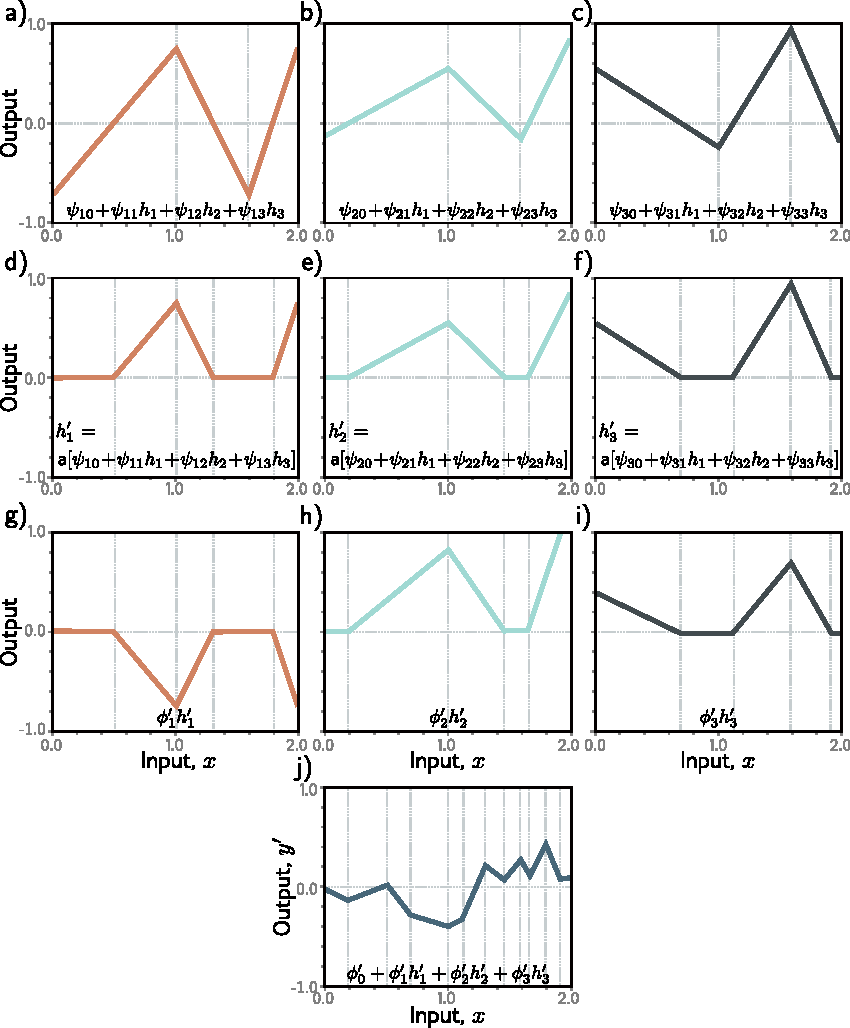
\includegraphics[height=0.65\textheight]{DeepBuildUp}
  \\[0.1em]
  \figsource{Prince (2023), Fig.~4.5: the two-layer network's
  output, built up layer by layer.}
\end{frame}

\begin{frame}{The general deep network}
  \begin{columns}[T, onlytextwidth]
    \begin{column}{0.55\textwidth}
      \centering
      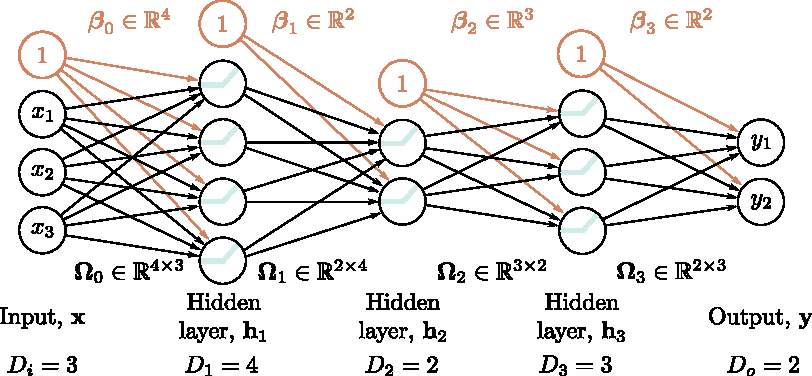
\includegraphics[width=\linewidth]{DeepKLayer}
      \\[0.1em]
      \figsource{Prince (2023), Fig.~4.6.}
    \end{column}
    \hfill
    \begin{column}{0.42\textwidth}
      \vspace{0.2em}
      {\small $K$ hidden layers, matrix notation:}
      \[
        \mathbf{h}_k = \mathrm{a}\big[\bm\beta_{k-1} +
        \bm\Omega_{k-1}\mathbf{h}_{k-1}\big]
      \]
      \begin{itemize}\setlength{\itemsep}{2pt}
        \item Weights $\bm\Omega_k$, biases
              $\bm\beta_k$ per layer
        \item \alert{Depth} $=$ number of hidden layers;
              \alert{width} $=$ units per layer
        \item Both are \alert{hyperparameters} --- chosen,
              not learned
      \end{itemize}
    \end{column}
  \end{columns}
  {\scriptsize\color{mcMuted} Prince (2023), Eqs.~4.15--4.16.}
\end{frame}

\begin{frame}{The same object in Bishop's notation}
  \begin{columns}[T, onlytextwidth]
    \begin{column}{0.5\textwidth}
      \centering
      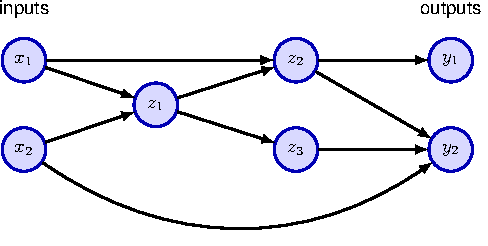
\includegraphics[width=0.86\linewidth]{Bishop6_15}
      \\[0.1em]
      \figsource{Bishop \& Bishop (2024), Fig.~6.15.}
    \end{column}
    \hfill
    \begin{column}{0.46\textwidth}
      \vspace{0.3em}
      \begin{itemize}\setlength{\itemsep}{2pt}
        \item A \alert{feedforward network}: information
              flows input $\to$ output, no cycles
        \item Each layer applies
              $\mathbf{z}^{(l)} = h\big(\mathbf{W}^{(l)}
              \mathbf{z}^{(l-1)}\big)$
        \item ``deep'' simply means \alert{more than one}
              hidden layer
              \hfill{\scriptsize Bishop \& Bishop, \S6.1}
      \end{itemize}
    \end{column}
  \end{columns}
  \shpar{single-layer NN / shallow net}
        {multi-layer / \alert{feedforward} network (FNN)}
\end{frame}

\begin{frame}{Building depth recursively}
  The two-layer construction \alert{extends recursively}
  (Bishop \& Bishop, 2024, \S6.2):
  \[
    \mathbf{z}^{(1)} = h\big(\mathbf{W}^{(1)}\mathbf{x}\big),
    \quad
    \mathbf{z}^{(2)} = h\big(\mathbf{W}^{(2)}\mathbf{z}^{(1)}\big),
    \quad \dots, \quad
    \mathbf{y} = f\big(\mathbf{W}^{(L)}\mathbf{z}^{(L-1)}\big)
  \]
  \begin{itemize}\setlength{\itemsep}{1pt}
    \item Each layer feeds the next --- the \alert{same
          operation} (linear map $+$ nonlinearity) repeated
    \item The construction extends recursively into a
          \alert{hierarchical model with many layers} --- the
          basis for deep networks
          \hfill{\scriptsize Bishop \& Bishop, \S6.2}
    \item Nothing new is needed --- depth is \alert{repetition
          of a single idea}
  \end{itemize}
  \shpar{$\mathbf{y} = \phi_0 + \bm\phi\,h(\mathbf{Wx})$}
        {$\mathbf{y} = f(\mathbf{W}^{(L)}h(\cdots
         h(\mathbf{W}^{(1)}\mathbf{x})))$}
\end{frame}

\begin{frame}{A note on counting layers}
  \begin{columns}[T, onlytextwidth]
    \begin{column}{0.44\textwidth}
      \centering
      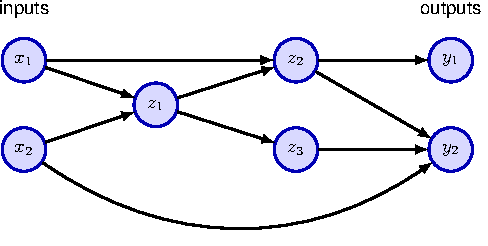
\includegraphics[width=0.92\linewidth]{Bishop6_15}
      \\[0.1em]
      \figsource{Bishop \& Bishop (2024), Fig.~6.15.}
    \end{column}
    \hfill
    \begin{column}{0.52\textwidth}
      \vspace{0.2em}
      {\small The same network is described inconsistently in
      the literature:}
      \begin{itemize}\setlength{\itemsep}{2pt}
        \item ``three-layer'' --- counting \emph{all} layers
              of units, inputs included
        \item ``single-hidden-layer'' --- counting only
              \emph{hidden} layers
        \item Bishop recommends counting \alert{layers of
              weights} (adaptive parameters)
              \hfill{\scriptsize Bishop \& Bishop, \S6.3}
      \end{itemize}
      {\small We will say a network is \alert{deep} when it
      has \alert{more than one} hidden layer.}
    \end{column}
  \end{columns}
\end{frame}

% =====================================================================
\section{What Deep Networks Represent}
% =====================================================================

\begin{frame}{Depth as an inductive bias}
  \begin{itemize}
    \item Universality tells us \emph{what} a network
          \emph{can} represent; it says nothing about what it
          \emph{prefers} to learn
    \item A deep architecture encodes an \alert{inductive
          bias}: that the output relates to the input through
          a \alert{hierarchy} of intermediate concepts
          \hfill{\scriptsize Bishop \& Bishop, \S6.3.1}
    \item For images, the map from pixels to a concept like
          `cat' is \alert{highly nonlinear} --- hopeless for
          one layer, natural for many
    \item The right bias means the network needs \alert{less
          data} and generalises better
  \end{itemize}
  \shpar{bias: output is one nonlinear map of the input}
        {bias: output is a \alert{hierarchy} of simpler maps}
\end{frame}

\begin{frame}{Hierarchical representations}
  \centering
  \begin{tikzpicture}[>=Stealth, line width=0.8pt,
      node distance=3mm,
      b/.style={rounded corners=3pt, draw=dpc, fill=dpc!7,
                align=center, minimum height=0.95cm,
                inner xsep=5pt, font=\small},
      lbl/.style={font=\scriptsize\itshape, mcMuted}]
    \node[b] (a) {pixels};
    \node[b, right=10mm of a] (b) {edges};
    \node[b, right=10mm of b] (c) {motifs\\ / parts};
    \node[b, right=10mm of c] (d) {objects};
    \node[b, right=10mm of d] (e) {`cat'};
    \draw[->] (a)--(b); \draw[->] (b)--(c);
    \draw[->] (c)--(d); \draw[->] (d)--(e);
    \node[lbl, below=1mm of a] {input};
    \node[lbl, below=1mm of b] {layer 1};
    \node[lbl, below=1mm of c] {layer 2};
    \node[lbl, below=1mm of d] {layer 3};
    \node[lbl, below=1mm of e] {output};
  \end{tikzpicture}
  \vspace{0.6em}
  \begin{itemize}\setlength{\itemsep}{2pt}
    \item Early layers detect \alert{low-level} features
          (edges, corners); later layers assemble them into
          \alert{high-level} concepts
    \item Each layer reuses the layer below --- features are
          \alert{shared} across everything built on top of
          them
    \item This compositional reuse is what one-layer networks
          cannot exploit
          \hfill{\scriptsize Bishop \& Bishop, \S6.3.1}
  \end{itemize}
\end{frame}

\begin{frame}{Why hierarchy is the right bias for real data}
  \begin{columns}[T, onlytextwidth]
    \begin{column}{0.46\textwidth}
      \centering
      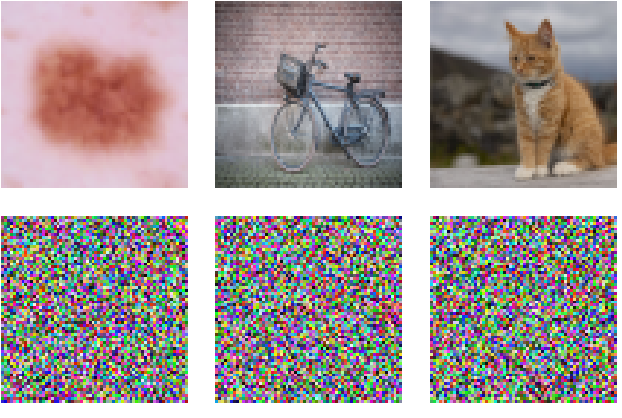
\includegraphics[width=0.86\linewidth]{Bishop6_8}
      \\[0.1em]
      \figsource{Bishop \& Bishop (2024), Fig.~6.8: natural
      images (top) vs.\ random pixels (bottom).}
    \end{column}
    \hfill
    \begin{column}{0.5\textwidth}
      \vspace{0.2em}
      \begin{itemize}\setlength{\itemsep}{2pt}
        \item Almost every random pixel pattern is
              \alert{noise} --- real images are vanishingly
              rare among all possible images
        \item Natural data lives on a \alert{low-dimensional
              manifold} with rich structure
        \item A hierarchy of features is exactly how to
              capture that structure efficiently ---
              \alert{compositional data, compositional model}
      \end{itemize}
    \end{column}
  \end{columns}
\end{frame}

\begin{frame}{Distributed representations}
  \begin{columns}[T, onlytextwidth]
    \begin{column}{0.44\textwidth}
      \centering
      \begin{tikzpicture}[line width=0.8pt, font=\scriptsize]
        \foreach \i/\lab in {0/fur,1/whiskers,2/round eyes,
                             3/pointy ears}{
          \node[circle, draw=dpc, fill=dpc!8, minimum size=6mm]
            (u\i) at (0,-\i*0.95) {};
          \node[right=1mm of u\i] {\lab};
        }
        \node[align=center, font=\scriptsize\itshape, mcMuted]
          at (1.1,-4.0) {a hidden layer};
      \end{tikzpicture}
    \end{column}
    \hfill
    \begin{column}{0.52\textwidth}
      \vspace{0.2em}
      \begin{itemize}\setlength{\itemsep}{2pt}
        \item Each unit signals whether a \alert{feature} is
              present (high) or absent (low)
        \item $M$ units name $M$ features --- but their
              \alert{combinations} can encode up to
              \alert{$2^M$} distinct patterns
        \item Concepts are represented by \alert{patterns of
              activity}, not single units --- a
              \alert{distributed} code
              \hfill{\scriptsize Bishop \& Bishop, \S6.3.2}
      \end{itemize}
    \end{column}
  \end{columns}
  \shpar{features fixed and hand-chosen}
        {features learned, and \alert{shared combinatorially}}
\end{frame}

\begin{frame}{Representation learning}
  \begin{columns}[T, onlytextwidth]
    \begin{column}{0.46\textwidth}
      \centering
      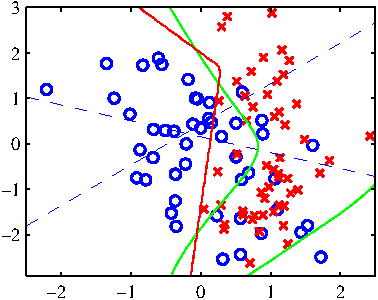
\includegraphics[width=0.76\linewidth]{Bishop6_11}
      \\[0.1em]
      \figsource{Bishop \& Bishop (2024), Fig.~6.11.}
    \end{column}
    \hfill
    \begin{column}{0.5\textwidth}
      \vspace{0.2em}
      \begin{itemize}\setlength{\itemsep}{1pt}
        \item Each layer \alert{transforms} the data to make
              the task easier
        \item By the final hidden layer, the classes are
              arranged so a \alert{simple linear classifier}
              separates them
        \item That layer's output is the \alert{learned
              representation} (embedding); the last layer just
              draws a line
              \hfill{\scriptsize Bishop \& Bishop, \S6.3.3}
      \end{itemize}
    \end{column}
  \end{columns}
  \shpar{one transform, then a linear read-out}
        {\emph{many} learned transforms, then a linear
         read-out}
\end{frame}

% =====================================================================
\section{Why Depth?}
% =====================================================================

\begin{frame}{Universal approximation, revisited}
  \begin{itemize}
    \item A shallow network is \alert{already} a universal
          approximator (Class~5) --- so why go deep?
    \item Because universality says a solution
          \alert{exists}, not that it is \alert{small}:
          matching a complex function may need exponentially
          many hidden units in one layer
    \item Deep networks can represent the same functions with
          \alert{far fewer parameters}
  \end{itemize}
  \vspace{0.3em}
  \begin{redhighlight}
    The question is not \emph{whether} but \emph{how
    efficiently} a network represents a function.
  \end{redhighlight}
\end{frame}

\begin{frame}{Linear regions per parameter}
  \begin{columns}[T, onlytextwidth]
    \begin{column}{0.58\textwidth}
      \centering
      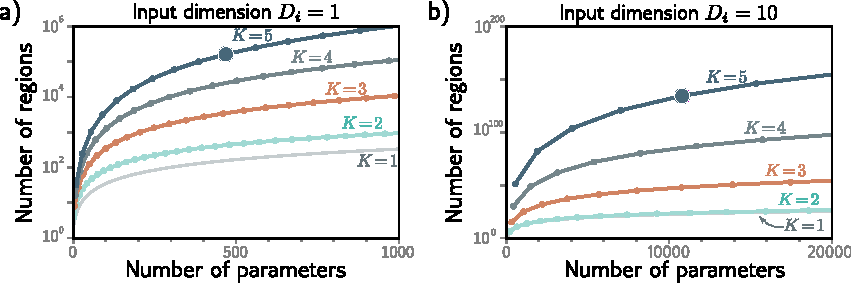
\includegraphics[width=\linewidth]{DeepParams}
      \\[0.1em]
      \figsource{Prince (2023), Fig.~4.7.}
    \end{column}
    \hfill
    \begin{column}{0.38\textwidth}
      \vspace{0.2em}
      \begin{itemize}\setlength{\itemsep}{1pt}
        \item Max linear regions vs.\ number of parameters
        \item For the same parameter budget, \alert{deeper}
              networks create \emph{far} more regions
        \item Depth grows expressivity
              \alert{multiplicatively}; width, only additively
      \end{itemize}
    \end{column}
  \end{columns}
  \shpar{regions grow \emph{polynomially} with width}
        {regions grow \emph{exponentially} with depth}
\end{frame}

\begin{frame}{Shallow vs.\ deep: the trade-off}
  \centering
  \renewcommand{\arraystretch}{1.2}
  {\small
  \begin{tabular}{p{0.26\textwidth} p{0.32\textwidth}
                  p{0.32\textwidth}}
    & \textbf{\color{shc}Shallow (1 layer)}
    & \textbf{\color{dpc}Deep (many layers)}\\
    \hline
    Expressivity & universal, but needs many units
      & universal with \alert{far fewer} units\\
    Regions & polynomial in width
      & exponential in depth\\
    Features & one level of learned features
      & \alert{hierarchical} features, layer on layer\\
    Training & convex read-out only
      & harder landscape; needs backprop (Class 11+)\\
    \hline
  \end{tabular}}
  \vspace{0.5em}
  \begin{redhighlight}
    Depth trades a harder optimisation problem for a
    dramatic gain in representational efficiency.
  \end{redhighlight}
\end{frame}

\begin{frame}{Why depth tends to win in practice}
  \begin{itemize}
    \item Real data is \alert{compositional}: edges $\to$
          shapes $\to$ objects; phonemes $\to$ words $\to$
          meaning
    \item Deep networks mirror this --- each layer builds
          \alert{features of the previous layer's features}
    \item Fewer parameters for the same function means
          \alert{better generalisation} and less data to fit
    \item Caveat: depth alone is not enough --- training deep
          networks needs the tools of the coming classes
          (initialisation, normalisation, residual
          connections)
  \end{itemize}
  \shpar{flat: features of the raw input}
        {hierarchical: features of features of features}
\end{frame}

\begin{frame}{Takeaways}
  \begin{enumerate}\setlength{\itemsep}{2pt}
    \item A \alert{deep network} is shallow networks
          \alert{composed}: each layer is a linear map
          followed by an activation
    \item Composition \alert{folds} input space, so regions
          \alert{multiply} across layers rather than add
    \item Both shallow and deep nets are universal ---
          but deep nets reach the same functions with
          \alert{exponentially fewer parameters}
    \item Depth suits \alert{compositional} data by building
          hierarchical features --- at the cost of a harder
          optimisation problem
  \end{enumerate}
  \vspace{0.3em}
  \begin{redhighlight}
    Next: depth and width efficiency theorems, then how to
    actually \alert{train} these networks (backpropagation).
  \end{redhighlight}
\end{frame}

\begin{frame}{References}
  \footnotesize
  \begin{itemize}
    \item S.~J.~D.~Prince. \textit{Understanding Deep
          Learning.} MIT Press, 2023. Chapter~4. Figures
          4.1--4.7 and teaching sequence from the author's
          repository (\url{https://udlbook.github.io/udlbook/}),
          CC BY-NC-ND, with attribution.
    \item C.~M.~Bishop \& H.~Bishop. \textit{Deep Learning:
          Foundations and Concepts.} Springer, 2024.
          Chapter~6. Figure 6.15 from the authors' published
          figure set, with attribution.
    \item G.~Cybenko (1989); K.~Hornik (1991);
          Montufar et al.\ (2014) on regions and depth.
  \end{itemize}
\end{frame}

\begin{frame}[standout]
  Questions?
\end{frame}

\end{document}
 